\documentclass{extbook}[14pt]
\usepackage{multicol, enumerate, enumitem, hyperref, color, soul, setspace, parskip, fancyhdr, amssymb, amsthm, amsmath, bbm, latexsym, units, mathtools}
\everymath{\displaystyle}
\usepackage[headsep=0.5cm,headheight=0cm, left=1 in,right= 1 in,top= 1 in,bottom= 1 in]{geometry}
\usepackage{dashrule}  % Package to use the command below to create lines between items
\newcommand{\litem}[1]{\item #1

\rule{\textwidth}{0.4pt}}
\pagestyle{fancy}
\lhead{}
\chead{Answer Key for Makeup Progress Quiz 1 Version C}
\rhead{}
\lfoot{6018-3080}
\cfoot{}
\rfoot{Spring 2021}
\begin{document}
\textbf{This key should allow you to understand why you choose the option you did (beyond just getting a question right or wrong). \href{https://xronos.clas.ufl.edu/mac1105spring2020/courseDescriptionAndMisc/Exams/LearningFromResults}{More instructions on how to use this key can be found here}.}

\textbf{If you have a suggestion to make the keys better, \href{https://forms.gle/CZkbZmPbC9XALEE88}{please fill out the short survey here}.}

\textit{Note: This key is auto-generated and may contain issues and/or errors. The keys are reviewed after each exam to ensure grading is done accurately. If there are issues (like duplicate options), they are noted in the offline gradebook. The keys are a work-in-progress to give students as many resources to improve as possible.}

\rule{\textwidth}{0.4pt}

\begin{enumerate}\litem{
Construct the lowest-degree polynomial given the zeros below. Then, choose the intervals that contain the coefficients of the polynomial in the form $ax^3+bx^2+cx+d$.
\[ 3, 1, \text{ and } \frac{7}{3} \]The solution is \( 3x^{3} -19 x^{2} +37 x -21 \), which is option A.\begin{enumerate}[label=\Alph*.]
\item \( a \in [1, 9], b \in [-19, -12], c \in [36, 42], \text{ and } d \in [-22, -19] \)

* $3x^{3} -19 x^{2} +37 x -21$, which is the correct option.
\item \( a \in [1, 9], b \in [-12, 4], c \in [-23, -22], \text{ and } d \in [21, 28] \)

$3x^{3} -1 x^{2} -23 x + 21$, which corresponds to multiplying out $(x + 3)(x -1)(3x -7)$.
\item \( a \in [1, 9], b \in [5, 11], c \in [-20, -16], \text{ and } d \in [-22, -19] \)

$3x^{3} +5 x^{2} -19 x -21$, which corresponds to multiplying out $(x + 3)(x + 1)(3x -7)$.
\item \( a \in [1, 9], b \in [-19, -12], c \in [36, 42], \text{ and } d \in [21, 28] \)

$3x^{3} -19 x^{2} +37 x + 21$, which corresponds to multiplying everything correctly except the constant term.
\item \( a \in [1, 9], b \in [9, 25], c \in [36, 42], \text{ and } d \in [21, 28] \)

$3x^{3} +19 x^{2} +37 x + 21$, which corresponds to multiplying out $(x + 3)(x + 1)(3x + 7)$.
\end{enumerate}

\textbf{General Comment:} To construct the lowest-degree polynomial, you want to multiply out $(x -3)(x -1)(3x -7)$
}
\litem{
Describe the end behavior of the polynomial below.
\[ f(x) = -2(x + 3)^{2}(x - 3)^{3}(x + 4)^{2}(x - 4)^{4} \]The solution is the graph below, which is option A.
\begin{center}
    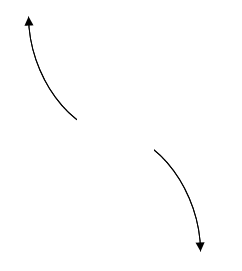
\includegraphics[width=0.3\textwidth]{../Figures/polyEndBehaviorAC.png}
\end{center}\begin{enumerate}[label=\Alph*.]
\begin{multicols}{2}
\item 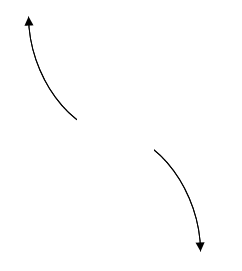
\includegraphics[width = 0.3\textwidth]{../Figures/polyEndBehaviorAC.png}
\item 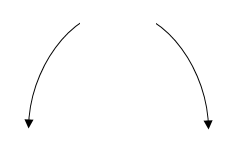
\includegraphics[width = 0.3\textwidth]{../Figures/polyEndBehaviorBC.png}
\item 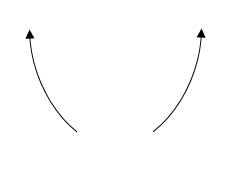
\includegraphics[width = 0.3\textwidth]{../Figures/polyEndBehaviorCC.png}
\item 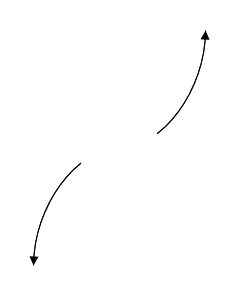
\includegraphics[width = 0.3\textwidth]{../Figures/polyEndBehaviorDC.png}
\end{multicols}\item None of the above.\end{enumerate}
\textbf{General Comment:} Remember that end behavior is determined by the leading coefficient AND whether the \textbf{sum} of the multiplicities is positive or negative.
}
\litem{
Construct the lowest-degree polynomial given the zeros below. Then, choose the intervals that contain the coefficients of the polynomial in the form $x^3+bx^2+cx+d$.
\[ -4 - 3 i \text{ and } 2 \]The solution is \( x^{3} +6 x^{2} +9 x -50 \), which is option D.\begin{enumerate}[label=\Alph*.]
\item \( b \in [-7.2, -5.5], c \in [6.8, 10.2], \text{ and } d \in [48.9, 50.9] \)

$x^{3} -6 x^{2} +9 x + 50$, which corresponds to multiplying out $(x-(-4 - 3 i))(x-(-4 + 3 i))(x + 2)$.
\item \( b \in [-0.8, 2.4], c \in [1.5, 2.3], \text{ and } d \in [-8.1, -6.2] \)

$x^{3} + x^{2} +2 x -8$, which corresponds to multiplying out $(x + 4)(x -2)$.
\item \( b \in [-0.8, 2.4], c \in [-0.7, 1.3], \text{ and } d \in [-7.9, -5.2] \)

$x^{3} + x^{2} +x -6$, which corresponds to multiplying out $(x + 3)(x -2)$.
\item \( b \in [2.7, 8.3], c \in [6.8, 10.2], \text{ and } d \in [-53.6, -47.8] \)

* $x^{3} +6 x^{2} +9 x -50$, which is the correct option.
\item \( \text{None of the above.} \)

This corresponds to making an unanticipated error or not understanding how to use nonreal complex numbers to create the lowest-degree polynomial. If you chose this and are not sure what you did wrong, please contact the coordinator for help.
\end{enumerate}

\textbf{General Comment:} Remember that the conjugate of $a+bi$ is $a-bi$. Since these zeros always come in pairs, we need to multiply out $(x-(-4 - 3 i))(x-(-4 + 3 i))(x-(2))$.
}
\litem{
Construct the lowest-degree polynomial given the zeros below. Then, choose the intervals that contain the coefficients of the polynomial in the form $ax^3+bx^2+cx+d$.
\[ \frac{7}{4}, \frac{-2}{3}, \text{ and } \frac{-4}{3} \]The solution is \( 36x^{3} +9 x^{2} -94 x -56 \), which is option B.\begin{enumerate}[label=\Alph*.]
\item \( a \in [35, 45], b \in [129, 138], c \in [152, 162], \text{ and } d \in [53, 59] \)

$36x^{3} +135 x^{2} +158 x + 56$, which corresponds to multiplying out $(4x + 7)(3x + 2)(3x + 4)$.
\item \( a \in [35, 45], b \in [9, 14], c \in [-96, -83], \text{ and } d \in [-56, -51] \)

* $36x^{3} +9 x^{2} -94 x -56$, which is the correct option.
\item \( a \in [35, 45], b \in [83, 91], c \in [10, 14], \text{ and } d \in [-56, -51] \)

$36x^{3} +87 x^{2} +10 x -56$, which corresponds to multiplying out $(4x + 7)(3x -2)(3x + 4)$.
\item \( a \in [35, 45], b \in [-10, 0], c \in [-96, -83], \text{ and } d \in [53, 59] \)

$36x^{3} -9 x^{2} -94 x + 56$, which corresponds to multiplying out $(4x + 7)(3x -2)(3x -4)$.
\item \( a \in [35, 45], b \in [9, 14], c \in [-96, -83], \text{ and } d \in [53, 59] \)

$36x^{3} +9 x^{2} -94 x + 56$, which corresponds to multiplying everything correctly except the constant term.
\end{enumerate}

\textbf{General Comment:} To construct the lowest-degree polynomial, you want to multiply out $(4x -7)(3x + 2)(3x + 4)$
}
\litem{
Construct the lowest-degree polynomial given the zeros below. Then, choose the intervals that contain the coefficients of the polynomial in the form $x^3+bx^2+cx+d$.
\[ 3 - 3 i \text{ and } -2 \]The solution is \( x^{3} -4 x^{2} +6 x + 36 \), which is option A.\begin{enumerate}[label=\Alph*.]
\item \( b \in [-8, 0], c \in [5.4, 8.1], \text{ and } d \in [35, 43] \)

* $x^{3} -4 x^{2} +6 x + 36$, which is the correct option.
\item \( b \in [2, 8], c \in [5.4, 8.1], \text{ and } d \in [-39, -29] \)

$x^{3} +4 x^{2} +6 x -36$, which corresponds to multiplying out $(x-(3 - 3 i))(x-(3 + 3 i))(x -2)$.
\item \( b \in [1, 2], c \in [-2.7, 2.2], \text{ and } d \in [-8, -2] \)

$x^{3} + x^{2} -x -6$, which corresponds to multiplying out $(x -3)(x + 2)$.
\item \( b \in [1, 2], c \in [4.6, 5.1], \text{ and } d \in [4, 8] \)

$x^{3} + x^{2} +5 x + 6$, which corresponds to multiplying out $(x + 3)(x + 2)$.
\item \( \text{None of the above.} \)

This corresponds to making an unanticipated error or not understanding how to use nonreal complex numbers to create the lowest-degree polynomial. If you chose this and are not sure what you did wrong, please contact the coordinator for help.
\end{enumerate}

\textbf{General Comment:} Remember that the conjugate of $a+bi$ is $a-bi$. Since these zeros always come in pairs, we need to multiply out $(x-(3 - 3 i))(x-(3 + 3 i))(x-(-2))$.
}
\litem{
Which of the following equations \textit{could} be of the graph presented below?

\begin{center}
    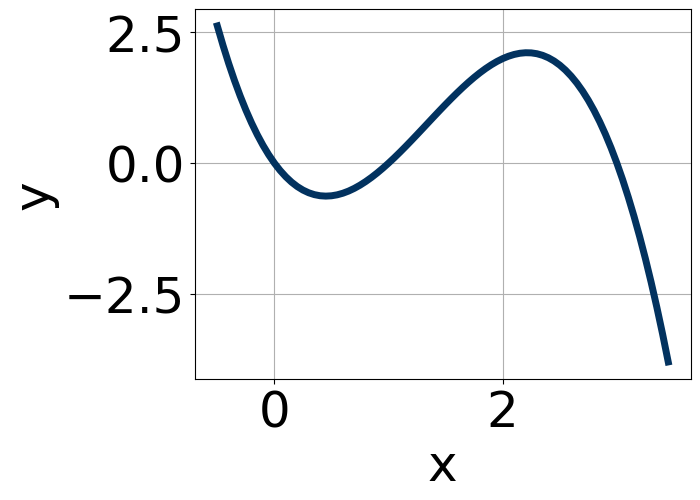
\includegraphics[width=0.5\textwidth]{../Figures/polyGraphToFunctionC.png}
\end{center}


The solution is \( -17x^{5} (x - 3)^{11} (x - 1)^{11} \), which is option B.\begin{enumerate}[label=\Alph*.]
\item \( -11x^{4} (x - 3)^{6} (x - 1)^{7} \)

The factors $0$ and $3$ have have been odd power.
\item \( -17x^{5} (x - 3)^{11} (x - 1)^{11} \)

* This is the correct option.
\item \( 8x^{10} (x - 3)^{9} (x - 1)^{5} \)

The factor $x$ should have an odd power and the leading coefficient should be the opposite sign.
\item \( 20x^{5} (x - 3)^{11} (x - 1)^{9} \)

This corresponds to the leading coefficient being the opposite value than it should be.
\item \( -10x^{8} (x - 3)^{5} (x - 1)^{5} \)

The factor $0$ should have been an odd power.
\end{enumerate}

\textbf{General Comment:} General Comments: Draw the x-axis to determine which zeros are touching (and so have even multiplicity) or cross (and have odd multiplicity).
}
\litem{
Describe the zero behavior of the zero $x = 8$ of the polynomial below.
\[ f(x) = -8(x + 3)^{12}(x - 3)^{8}(x + 8)^{6}(x - 8)^{3} \]The solution is the graph below, which is option A.
\begin{center}
    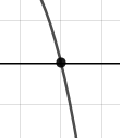
\includegraphics[width=0.3\textwidth]{../Figures/polyZeroBehaviorCopyAC.png}
\end{center}\begin{enumerate}[label=\Alph*.]
\begin{multicols}{2}
\item 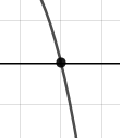
\includegraphics[width = 0.3\textwidth]{../Figures/polyZeroBehaviorCopyAC.png}
\item 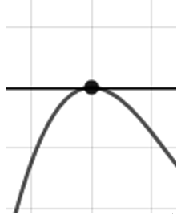
\includegraphics[width = 0.3\textwidth]{../Figures/polyZeroBehaviorCopyBC.png}
\item 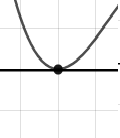
\includegraphics[width = 0.3\textwidth]{../Figures/polyZeroBehaviorCopyCC.png}
\item 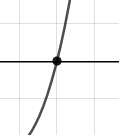
\includegraphics[width = 0.3\textwidth]{../Figures/polyZeroBehaviorCopyDC.png}
\end{multicols}\item None of the above.\end{enumerate}
\textbf{General Comment:} You will need to sketch the entire graph, then zoom in on the zero the question asks about.
}
\litem{
Describe the end behavior of the polynomial below.
\[ f(x) = -3(x + 3)^{2}(x - 3)^{3}(x + 2)^{5}(x - 2)^{7} \]The solution is the graph below, which is option A.
\begin{center}
    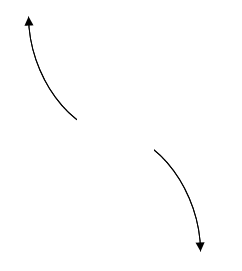
\includegraphics[width=0.3\textwidth]{../Figures/polyEndBehaviorCopyAC.png}
\end{center}\begin{enumerate}[label=\Alph*.]
\begin{multicols}{2}
\item 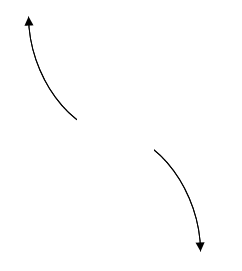
\includegraphics[width = 0.3\textwidth]{../Figures/polyEndBehaviorCopyAC.png}
\item 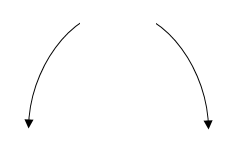
\includegraphics[width = 0.3\textwidth]{../Figures/polyEndBehaviorCopyBC.png}
\item 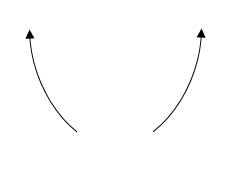
\includegraphics[width = 0.3\textwidth]{../Figures/polyEndBehaviorCopyCC.png}
\item 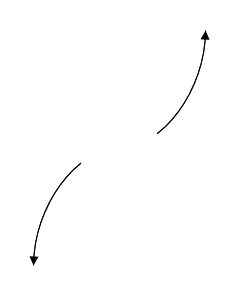
\includegraphics[width = 0.3\textwidth]{../Figures/polyEndBehaviorCopyDC.png}
\end{multicols}\item None of the above.\end{enumerate}
\textbf{General Comment:} Remember that end behavior is determined by the leading coefficient AND whether the \textbf{sum} of the multiplicities is positive or negative.
}
\litem{
Which of the following equations \textit{could} be of the graph presented below?

\begin{center}
    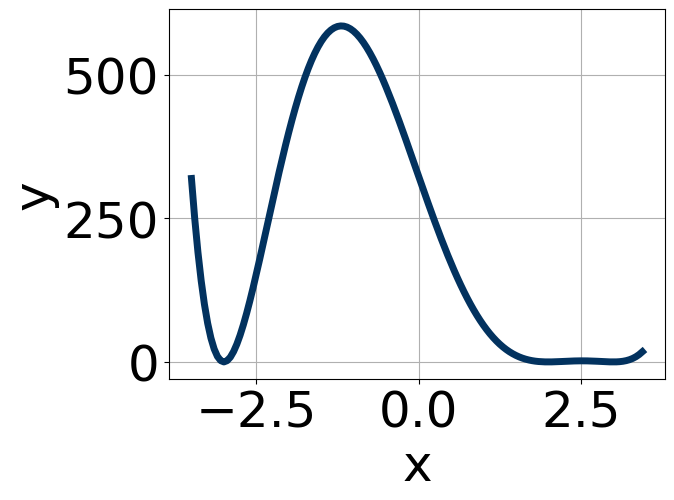
\includegraphics[width=0.5\textwidth]{../Figures/polyGraphToFunctionCopyC.png}
\end{center}


The solution is \( 17(x + 3)^{10} (x - 3)^{6} (x - 2)^{8} \), which is option A.\begin{enumerate}[label=\Alph*.]
\item \( 17(x + 3)^{10} (x - 3)^{6} (x - 2)^{8} \)

* This is the correct option.
\item \( -18(x + 3)^{10} (x - 3)^{10} (x - 2)^{11} \)

The factor $(x - 2)$ should have an even power and the leading coefficient should be the opposite sign.
\item \( -18(x + 3)^{10} (x - 3)^{4} (x - 2)^{4} \)

This corresponds to the leading coefficient being the opposite value than it should be.
\item \( 10(x + 3)^{4} (x - 3)^{7} (x - 2)^{5} \)

The factors $(x - 3)$ and $(x - 2)$ should both have even powers.
\item \( 4(x + 3)^{4} (x - 3)^{4} (x - 2)^{5} \)

The factor $(x - 2)$ should have an even power.
\end{enumerate}

\textbf{General Comment:} General Comments: Draw the x-axis to determine which zeros are touching (and so have even multiplicity) or cross (and have odd multiplicity).
}
\litem{
Describe the zero behavior of the zero $x = 4$ of the polynomial below.
\[ f(x) = 4(x + 9)^{4}(x - 9)^{2}(x + 4)^{13}(x - 4)^{8} \]The solution is the graph below, which is option C.
\begin{center}
    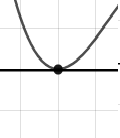
\includegraphics[width=0.3\textwidth]{../Figures/polyZeroBehaviorCC.png}
\end{center}\begin{enumerate}[label=\Alph*.]
\begin{multicols}{2}
\item 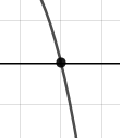
\includegraphics[width = 0.3\textwidth]{../Figures/polyZeroBehaviorAC.png}
\item 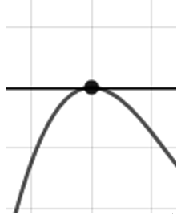
\includegraphics[width = 0.3\textwidth]{../Figures/polyZeroBehaviorBC.png}
\item 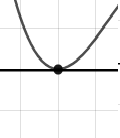
\includegraphics[width = 0.3\textwidth]{../Figures/polyZeroBehaviorCC.png}
\item 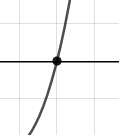
\includegraphics[width = 0.3\textwidth]{../Figures/polyZeroBehaviorDC.png}
\end{multicols}\item None of the above.\end{enumerate}
\textbf{General Comment:} You will need to sketch the entire graph, then zoom in on the zero the question asks about.
}
\end{enumerate}

\end{document}